\documentclass[12pt, twoside]{book}

% variable values
\input variables.tex

\ifshowframe{}
    \usepackage[a4paper,top=2.5cm,bottom=2.5cm,left=3.5cm,right=2cm,showframe]{geometry}
\else
    \usepackage[a4paper,top=2.5cm,bottom=2.5cm,left=3.5cm,right=2cm]{geometry}
\fi
\usepackage{microtype}
\usepackage[slovak,USenglish]{babel}
\usepackage[utf8]{inputenc}
\usepackage[T1]{fontenc}

\linespread{1.25} % this means 1.5 line spacing

% more package imports and custom commands
\input definitions.tex

\tikzset{every node/.style={circle, draw, fill=black}}

\begin{document}

\ifenglish{}
    \selectlanguage{USenglish}
\else
    \selectlanguage{slovak}
\fi

\frontmatter
\pagenumbering{gobble}

% COVER
\thispagestyle{empty}

{
    \sc\large

    \begin{center}
        \thesisuniversity{}\\
        \thesisfaculty{}

        \vfill

        {\LARGE\thesisname}\\
        \thesistype{}
    \end{center}

    \vfill

    \noindent
    \thesisyear{}\\
    \thesisauthor{}
}

\cleardoublepage{}

% TITLE PAGE
\frontmatter
\thispagestyle{empty}

\begin{center}
    \sc\large
    \thesisuniversity{}\\
    \thesisfaculty{}

    \vfill

    {\LARGE\thesisname}\\
    \thesistype{}
\end{center}

\vfill

\noindent
\begin{tabular}{ll}
    \ifenglish{}Study Programme:\else{}Študijný program:   \fi & \thesisprogramme{}\\
    \ifenglish{}Field of Study: \else{}Študijný odbor:     \fi & \thesisfield{}\\
    \ifenglish{}Department:     \else{}Školiace pracovisko:\fi & \thesisdepartment{}\\
    \ifenglish{}Supervisor:     \else{}Školiteľ:           \fi & \thesissupervisor{}\\
    \ifconsultant{}\ifenglish{}Consultant:\else{}Konzultant:\fi & \thesisconsultant{}\\ \fi
\end{tabular}

\vfill

\noindent
\thesislocation, \thesisyear{}\\
\thesisauthor{}

\cleardoublepage{}

% ASSIGNMENT
\newpage
\thispagestyle{empty}

\noindent
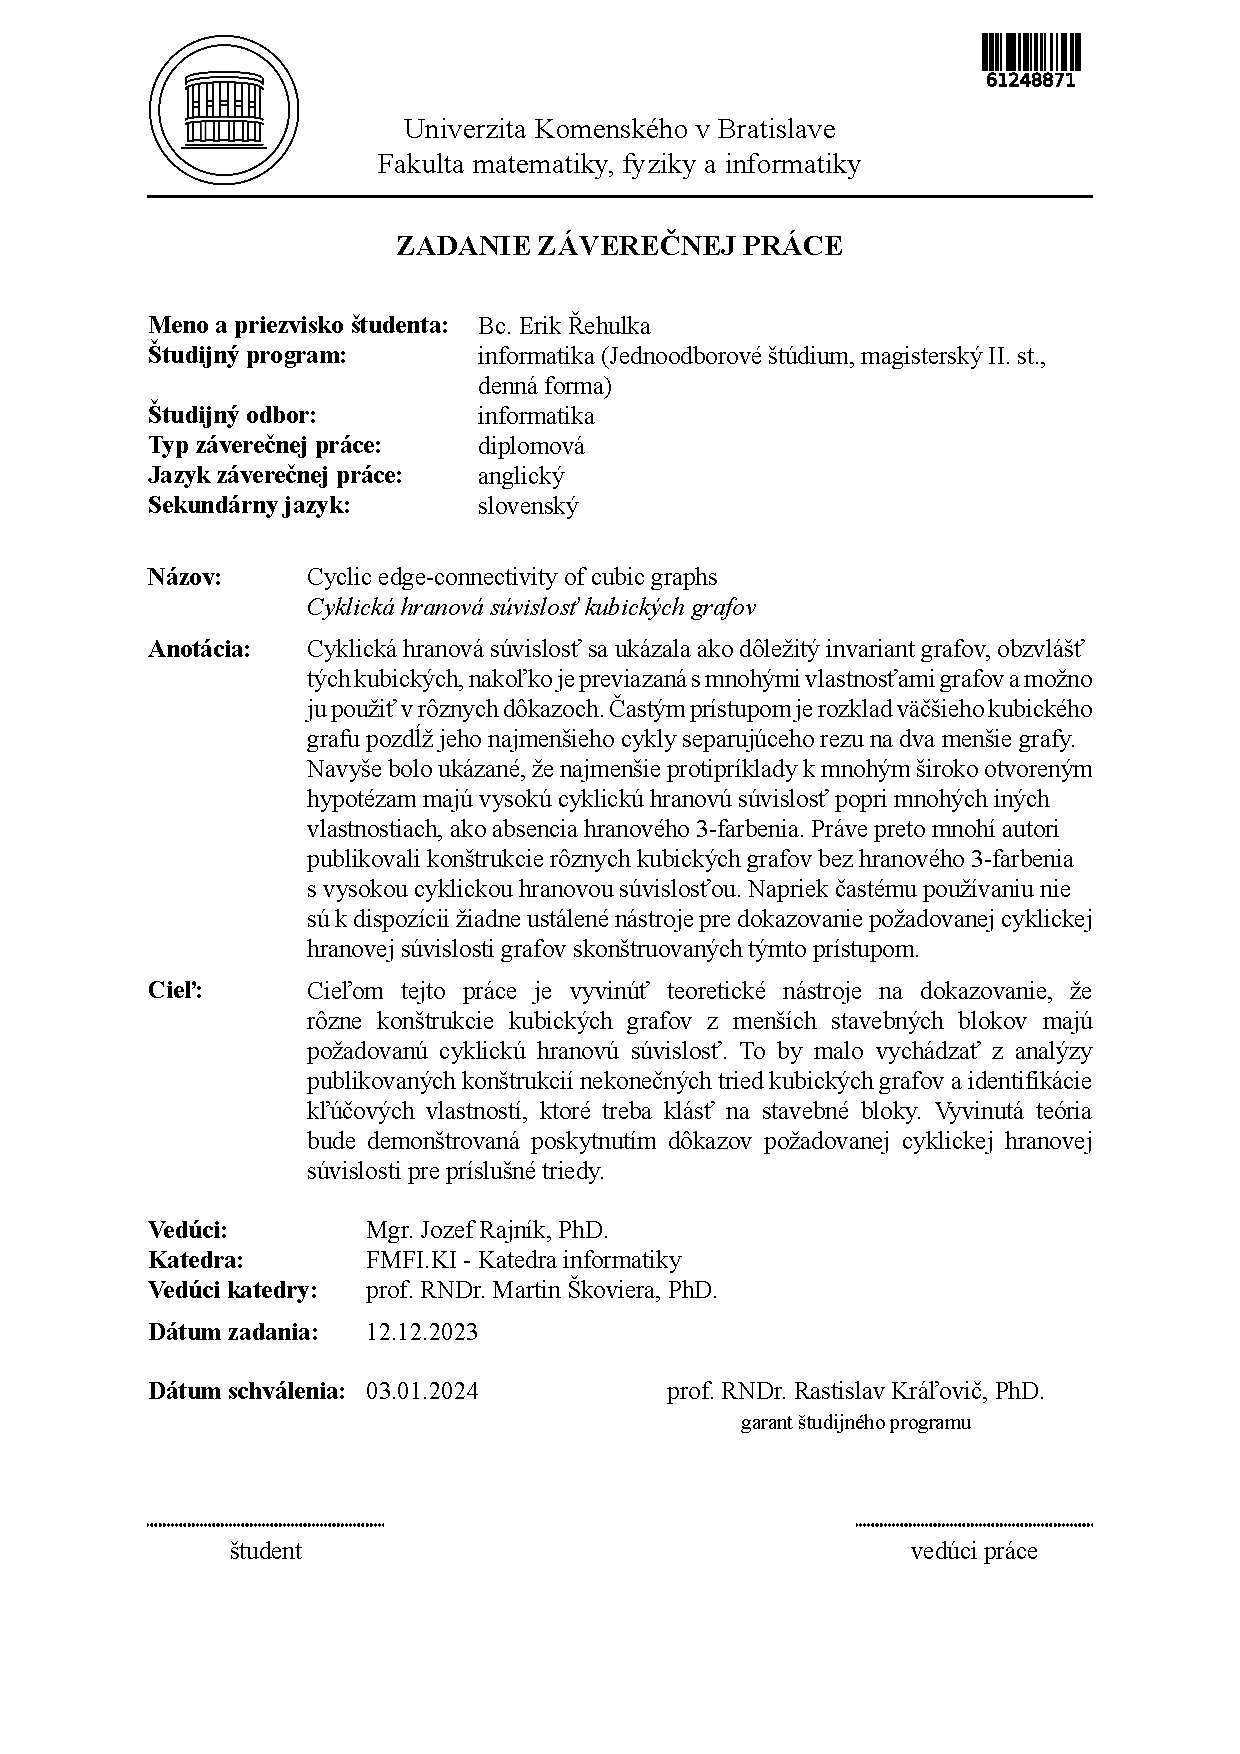
\includegraphics[trim=2.5cm 5cm 2.5cm 0,width=\textwidth]{images/assignment-sk.pdf}

\ifenglish{}
    \newpage
    \thispagestyle{empty}

    \noindent
    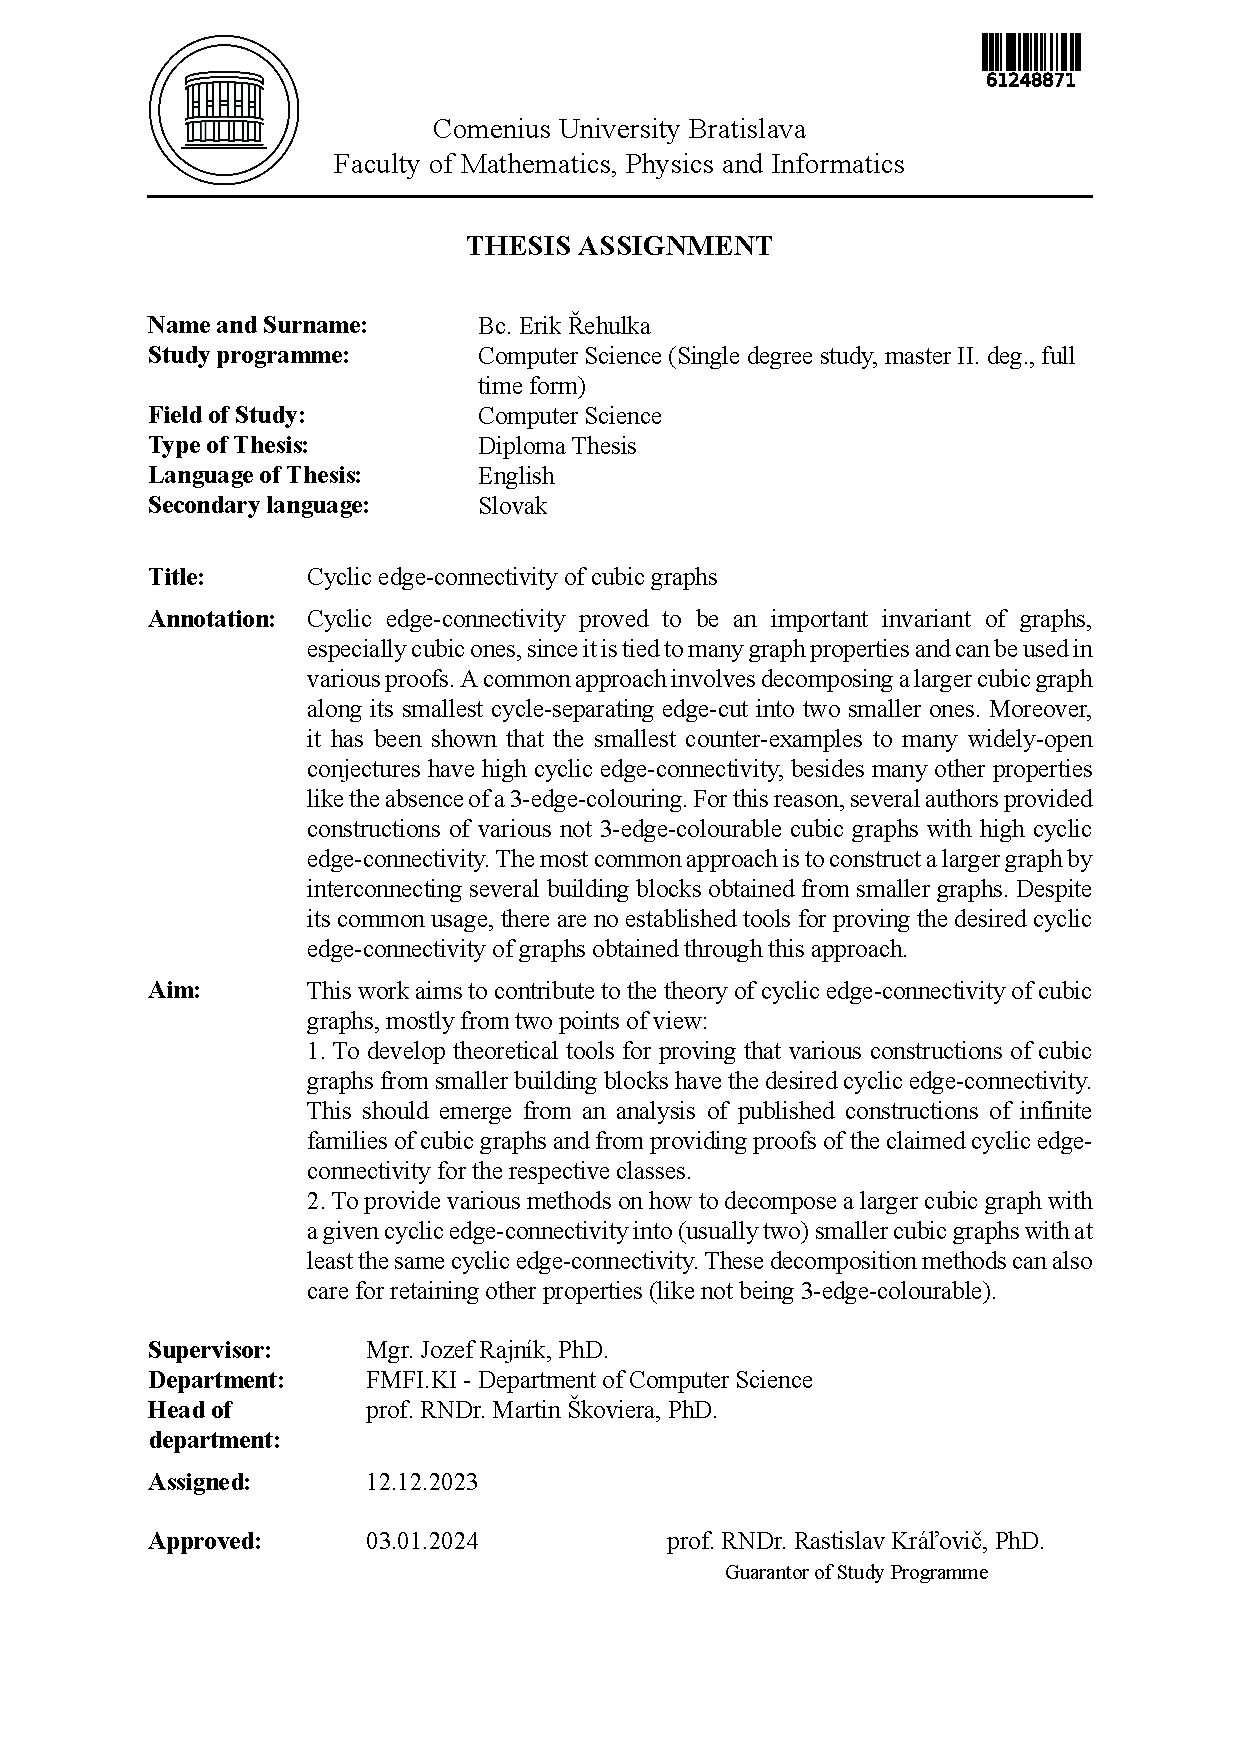
\includegraphics[trim=2.5cm 5cm 2.5cm 0,width=\textwidth]{images/assignment-en.pdf}
\fi

% ACKNOWLEDGEMENTS
\newpage

~\vfill
\paragraph*{\ifenglish{}Acknowledgments:\else{}Poďakovanie:\fi} \thesisacknowledgments{}

% ABSTRACT SK
\newpage

\begin{otherlanguage}{slovak}
    \section*{Abstrakt}

    \thesisabstractsk{}

    \paragraph*{Kľúčové slová:} \thesiskeywordssk{}
\end{otherlanguage}

% ABSTRACT EN
\newpage

\begin{otherlanguage}{USenglish}
    \section*{Abstract}

    \thesisabstracten{}

    \paragraph*{Keywords:} \thesiskeywordsen{}
\end{otherlanguage}

% TABLE OF CONTENTS, LIST OF FIGURES
\newpage
\tableofcontents

\newpage
\listoffigures

% CONTENTS
\mainmatter{}

\chapter*{Introduction}
\addcontentsline{toc}{chapter}{Introduction}
\markboth{Introduction}{Introduction}

\chapter{Preliminaries}\label{ch:preliminaries}

\section{Basic notions}

Definitions not provided in our work can be found in the book \quotes{Graph Theory} by Diestel \cite{Diestel}. All graphs considered in this work are undirected and finite. We do not allow trivial graphs, but sometimes for the sake of complete definition we address them. We permit multiple edges, as well as loops.

A \textit{girth} of a graph $G$, denoted by $g(G)$ is the minimum length of a cycle in $G$. If $G$ does not contain a cycle, we set the girth to $\infty$.

The distance between two vertices $x$ and $y$ in a graph $G$, denoted by $d_G(x,y)$, is defined as the length of the shortest path between $x$ and $y$ in $G$. If no such path exists, we set $d_G(x,y)=\infty$. If the specific graph $G$ is evident from the context, we shall only use $d(x,y)$.

While we work only with cyclic connectivity, for the sake of providing the definition completely in our work, we shall start with definining how we will compute connectivity, but more importantly, how we will work with edge cuts.

\section{Multipoles}\label{sec:multipoles}

In our work, we allow a specific type of graph, which allows ends of its edges to not be incident with a vertex, resulting in a graph with dangling, or even so-called isolated edges. Such structures are called \textit{multipoles}. This term was first used by Fiol in 1991 \cite{Fiol1991}, however we will be following a definition by Nedela and Škoviera \cite{Nedela1996}.

\begin{definition}[\cite{Nedela1996}]
	A \textit{multipole} is a pair $M=(V,E)$ of distinct finite sets of vertices $V$ and edges $E$, where every edge $e\in E$ has two edge ends, which may or need not be incident with a vertex.
	
	According to the incidence of edge ends, we define four types of edges:
	\begin{enumerate}[nolistsep]
		\item A \textit{link} is an edge whose ends are incident with two distinct vertices.
		\item A \textit{loop} is an edge whose ends are incident with the same vertex.
		\item A \textit{dangling edge} is an edge whose one end is incident with a vertex, and the other is not.
		\item An \textit{isolated edge} is an edge whose both ends are not incident with any vertex.
	\end{enumerate}
\end{definition}

A \textit{semiedge} is an edge end not incident with any vertex. For a given multipole $M$, we define $S(M)$ to be the tuple containing all the semiedges in that multipole. A multipole is connected if there exists a path between each pair of semiedges. It can be observed that if a multipole contains an isolated edge it is not connected.

A multipole $M$ with $n$ semiedges and $S(M) = (a_1, \cdots, a_n)$ can also be denoted as $M(a_1,\cdots,a_n)$. Similarly to graphs, the \textit{order} of a multipole $M$, denoted by $|M|$, is the number of its vertices. Also the \textit{degree} of a vertex $v$ of a multipole, denoted by $\deg(v)$, is the number of edge ends incident with $v$. A multipole with $k$ semiedges is usually called a \textit{k-pole}. It can be seen, that a graph can be defined as a 0-pole.

One of the features of multipoles is connecting them to form bigger multipoles or even graphs. They can be seen as small building blocks for constructing larger graphs or multipoles. 

Now, let $e$ and $f$ be edges (not necessarily distinct) and $e',~f'$ two of their semiedges respectively, such that $e'\neq f'$. If $e\neq f$, the result of the \textit{junction} of $e'$ and $f'$ is a new edge, having the other edge ends of $e$ and $f$ and a deletion of $e$ and $f$. If $e=f$, the result of the \textit{junction} of $e'$ and $f'$ is just the deletion of the edge.

The junction of two $k$-poles $M(a_1,\dots,a_k)$ and $N(b_1,\dots,b_k)$ consists of $k$ individual junctions of semiedges $a_i$ and $b_{f(i)}$, for $i$ from $1$ to $k$ and a bijection $f:\{1,\dots,k\}\rightarrow\{1,\dots,k\}$. We denote the junction as $M*_fN$, if we use an arbitrary bijection we simply denote it as $M*N$.

Consider two multipoles $M(a_1,\cdots,a_n)$ and $N(b_1,\cdots,b_m)$. Their \textit{partial junction of size $k$} is a junction of some semiedges $(a_{i_1},\cdots, a_{i_k})$ and $(b_{j_1},\cdots, b_{j_k})$, where $k\leq n$ and $k\leq m$. In contrast to a normal junction, which results in a graph, the partial junction can still result in a multipole. However we allow in partial junction the junction of all semiedges, thus a junction is a special case of partial junction where the result is a graph.

We say that a multipole $M$ contains a multipole $N$, or simply $N$ is in $M$ when there exists a multipole $P$ and a partial junction $*$ such that $N=M*P$

Same as in graphs, a multipole is cyclic if it contains a path which starts and ends in the same vertex, thus contains a cycle.

The distance between two semiedges $a$ and $b$ is equal to
\begin{itemize}
	\item 0 if both are part of the same edge,
	\item $\infty$ if at least one of $a,b$ is in an isolated edge,
	\item $d(x,y)$ where $x$ and $y$ are the vertices with which are incident the edges containing $a$ and $b$, respectively.
\end{itemize}

Since we allow these dangling and isolated edges, we can introduce so-called \textit{edge severing}. By severing an edge $e=e_1e_2$, we mean the removal of $e$, along with adding two new edges: $e_1e_3$ and $e_4e_2$, where $e_3$ and $e_4$ are new edge ends. It is evident that by severing a link we obtain two new dangling edges, by severing a dangling edge we obtain a new dangling edge and an isolated edge, and by severing an isolated edge we obtain two new isolated edges. In our work this also applies to cuts. When we say that and edge has been \textit{cut}, it means it has been severed.

Even though edges as we know them from graphs are denoted as links or loops in multipoles, we will keep calling them edges from now on. The reason is that we want to showcase the difference between edges which connect two (not necessarily distinct) vertices, and edges which have at least one end not incident with a vertex. Because of this when we will mention an edge in a multipole from now on, we mean a link or a loop in that multipole. We only differ from these edges by mentioning the separate semiedges, we do not need to differ between dangling and isolated edges.

\section{Edge Cuts and Connectivity}\label{sec:edge-cuts}

As the name suggests, an \textit{edge cut} decomposes a graph into multiple connected components. It is a set of edges of a graph $G$, such that if we sever every edge in the set, the resulting graph will not be connected. There is also a second way to denote an edge cut, which is helpful when trying to determine how will the vertices be split after severing the edges. Note that by $E(V_1,V_2)$ we denote the set of edges, which have one end in $V_1$ and the other in $V_2$.

Let $G$ be a graph and ${V_1,V_2}$ a partition of $V(G)$, such that both sets are non-empty. By $E(V_1,V_2)$ we denote the set of edges, which have one end in $V_1$ and the other in $V_2$.

Note, that $E(V_1,V_2)$ is indeed an edge cut, when we sever all of these edges, there will not be any edge between a vertex in $V_1$ and $V_2$, splitting the graph into two components. The sets $V_1$ and $V_2$ are called the sides of the cut.

A graph which results from a graph $G$ by severing edges from a set $S$ is denoted as $G-S$. Note that this does not require $S$ to be an edge cut, the result can still be connected.

A graph $G$ is \textit{k-edge-connected} (for $k\in\mathbb{N}$), if $|G|>k$ and $G-S$ is connected for every set $S\subseteq E(G)$ such that $|S|<k$. In other words, there is no edge cut with less than $k$ edges.

\begin{definition}
	Let $G$ be a graph. The \textit{edge conectivity} of $G$, denoted by $\lambda(G)$ is the greatest $k\in\mathbb{N}$ such that $G$ is $k$-edge-connected.
\end{definition}

In other words, it is the size of the smallest edge cut in the graph. It can be easily proven, that for each non-trivial graph $G$ it holds that $\lambda(G)\leq\delta(G)$. The proof comes from the fact, that all edges incident with a vertex are indeed edge cuts, separating the vertex from the rest of the graph, meaning there is an edge cut of size $\delta(G)$ in each graph. Also it holds that if $G$ is disconnected, $\lambda(G)=0$.

\section{Vertex connectivity}

In vertex connectivity we do not cut or remove edges, but remove vertices. By removing a vertex in a multipole $M$ we mean removing this vertex along with all of its incident edges \todo{NIE! Chceme pridať visiace hrany!}. A \textit{vertex cut} is in that case a subset of vertices of $G$, such that after their removal we obtain a disconnected graph.

A graph $G$ is called \textit{k-connected} for $k\in\mathbb{N}$ if $|G|>k$ and $G-X$ is connected for every subset $X\subseteq V(G)$ with $|X|<k$. In other words, there is no vertex cut in $G$ with less than $k$ semiedges. We can also specify that it is connected to vertex conectivity by denoting it as \textit{k-vertex-connected}, however in our work we use only the first name.

Similarly to edge connectivity, a \textit{vertex connectivity}, or just connectivity of $G$, denoted by $\kappa(G)$, is the greatest integer $k$ such that $G$ is $k$-connected.

Note that we can use the same argument for the upper bound of $\kappa(G)$ being $\delta(G)$, since we can just select a vertex with the minimal degree, and its neighbors will be a vertex cut, excluding loops to not remove the selected vertex. The only difference is in complete graphs, where from the definition the connectivity of $K_n$ is $n-1$, since no set of vertices represents a vertex cut, however $\delta(K_n)=n-1$, thus this also holds. In comparison with edge-connectivity, in nontrivial graphs for each such graph $G$ it holds that $\kappa(G)\leq \lambda(G) \leq \delta(G)$.

\section{Cyclic Edge Connectivity}\label{sec:cyclic-edge-connectivity}

The fact that  can be a huge limitation, since for example when trying to explore cubic graphs, the upper bound of the edge connectivity is three. Because of this, a new metrics regarding edge cuts were introduced, requiring both of the components resulting after severing edges from an edge cut to contain cycles. The notation is similar as before, just with a keyword \textit{cyclic} before it. To maintain a reasonable level of formalism, we shall define these properties more precise.

An edge cut $E(V_1,V_2)$ in a graph $G$ is called \textit{cycle separating}, if both induced subgraphs $G[V_1]$ and $G[V_2]$ contain a cycle. In contrast to edge cuts, there are non-trivial graphs which do not contain a cycle separating edge cut \cite{atoms-of-cyclic, Lou2008, lovasz1965graphs}, for example trees. In cubic graphs however, there are only three of such graphs: $K_{3,3}, K_4, \Theta_2$ \cite{atoms-of-cyclic} visible in \cref{fig:graphs-k33-k4-theta2}.

\begin{figure}
	\centering
	\begin{subfigure}[c]{0.3\textwidth}
		\centering
		\begin{tikzpicture}[baseline]
			% Define nodes for the left side (A)
			\foreach \x in {1,2,3}
			\node (A\x) at (\x,0) {};
			
			% Define nodes for the right side (B)
			\foreach \y in {1,2,3}
			\node (B\y) at (\y,-2) {};
			
			% Draw edges between the nodes
			\foreach \x in {1,2,3}
			\foreach \y in {1,2,3}
			\draw (A\x) -- (B\y);
		\end{tikzpicture}
	\end{subfigure}%
	\begin{subfigure}[c]{0.3\textwidth}
		\centering
		\begin{tikzpicture}[baseline]
			% Define vertices
			\node (A) at (0,2) {};
			\node (B) at (2,2) {};
			\node (C) at (2,0) {};
			\node (D) at (0,0) {};
			
			% Draw edges
			\draw (A) -- (B);
			\draw (A) -- (C);
			\draw (A) -- (D);
			\draw (B) -- (C);
			\draw (B) -- (D);
			\draw (C) -- (D);
		\end{tikzpicture}
	\end{subfigure}%
	\begin{subfigure}[c]{0.3\textwidth}
		\centering
		\begin{tikzpicture}[baseline]
			\node (A) at (0,0) {};
			\node (B) at (2,0) {};
			
			% Three parallel edges with different curvatures
			\draw (A) to[bend left=30] (B);
			\draw (A) -- (B);
			\draw (A) to[bend right=30] (B);
		\end{tikzpicture}
	\end{subfigure}
	\caption{Graphs $K_{3,3},K_4$ and $\Theta_2$}
	\label{fig:graphs-k33-k4-theta2}
\end{figure}

Similarly to edge connectivity, we say that graph $G$ is \textit{cyclically k-edge-connected}, if there is no cycle separating edge cut with less than $k$ edges.

Let $\beta(G)=|E|-|V|+1$ be the cycle rank of $G$. Deleting any set of $k\geq \beta(G)$ yields either a disconnected graph or a graph without cycles, thus if $G$ contains a cycle separating edge cut, it must contain one with no more than $\beta(G)-1$ edges \cite{atoms-of-cyclic}.

\begin{definition}[\cite{atoms-of-cyclic}]
	Let $G$ be a graph. The \textit{cyclic edge conectivity} of $G$, denoted by $\zeta(G)$ is the largest integer $k \leq \beta(G)$ such that $G$ is cyclically $k$-edge-connected.
\end{definition}

This means, that if a graph $G$ does not contain a cycle separating edge cut, its cyclic edge connectivity is equal to $\beta(G)$. Note that for acyclic graphs this number is 0, for the three mentioned cubic graphs the values are $\zeta(K_{3,3})=4, \zeta(K_4)=3, \zeta(\Theta_2)=2$.

More properties of cyclic edge connectivity are regarded in \cref{ch:cyclic-edge-connectivity}.

\section{Transitive graphs}\label{sec:transitive-graphs}

In proving the results of our work, we have used so-called \textit{Cayley graphs}, for which there are some proved theorems and can be helpful with their properties for our results. To properly define them, we need to dive a bit into an algebraic graph theory, and prove what it means for a graph to be transitive. All of these definitions were taken from a book by Godsil and Royle \cite{algebraic-graph-theory}.

An automorphism on a graph $G$ is an isomorphism from $G$ to itself, in other words a permutation of the vertices of $G$ that maps edges to edges and nonedges to nonedges. Trivial case of an automorphism is an identity permutation. It holds that the set of all automorphisms of $G$ forms a group.

A graph $G$ is called vertex-transitive if for any two vertices $x,y\in V(G)$ there is an automorphism of $G$ mapping $x$ to $y$. Similarly, it is called edge-transitive if for any two edges $e,f$ there is an automorphism of $G$ that maps $e$ to $f$. It must be noted that these properties are not equivalent. If a graph is edge-transitive, it does not have to be vertex-transitive. Take for example complete bipartite graph $K_{m,n}$ where $m\neq n$. They are edge transitive, however they can not be vertex transitive, since no automorphism can map a vertex of degree $m$ to a vertex of degree $n$ where $m\neq n$.

A vertex-transitive connected graph $G$ is called Cayley if it has a group $\Gamma$ of automorphisms such that for all $u, v \in V(G)$ there exists exactly one automorphism $\phi\in\Gamma$ such that $\phi(u)=v$. In other words, $\Gamma$ acts regularly on $V(G)$. The fact that there is a family of vertex-transitive graphs is very helpful for proving subsequent theorems, since cyclic-edge connectivity is interesting to explore on vertex-transitive graphs. For now we shall mention the following theorem about the existence of $k$-regular vertex-transitive graph with arbitrary girth and $k$, which we will use to construct cubic vertex-transitive graphs.

\begin{theorem}[\cite{small-vertex-transitive}]\label{th:cayley-girth-regular}
	For every pair of parameters $k \geq 2, g \geq 3$, there exists a finite $k$-regular Cayley graph $C(\Gamma, X)$ of girth $g$.
\end{theorem}

Thus there is a cubic vertex-transitive graph of arbitrary girth.

\chapter{Cyclic Edge Connectivity}\label{ch:cyclic-edge-connectivity}

From this chapter, all of the used graphs and multipoles will be cyclic, if not stated otherwise.

\begin{proposition}[{{\cite[Proposition 2]{atoms-of-cyclic}}}]\label{prop:cyclic-con-less-than-girth}
	For every connected cubic graph $G$ it holds that $\zeta(G)\leq g(G)$.
\end{proposition}

\section{Cyclic Vertex Connectivity}

\todo{} tu definuj najskôr vertex cut, následne čo je cyclic vertex connectivity, potom hentú vetu o ekvivalencii (na ňu sa potom môžeš odvolať) a uzavri to že vlastne je to rovnaké v kubických grafoch tak to je vlastne OK.

\begin{theorem}[{{\cite{atoms-of-cyclic,mccuaig-edge-reductions}}}]
	Let $G$ be a connected cubic graph not isomorphic to $K_{3,3},K_4$ or $\Theta_2$. Then the following conditions are equivalent:
	\begin{enumerate}
		\item $G$ is cyclically $k$-edge-connected,
		\item $G$ is cyclically $k$-vertex-connected,
		\item Each independent edge cut has at least $k$ edges.
	\end{enumerate}
\end{theorem}

\section{Cyclic parts}\label{sec:cyclic-parts}

\begin{definition}
	Let $G$ be a graph and let $X$ be a minimum cycle separating edge cut in $G$. Then the components which arise after cutting $X$ in $G$ are called \textit{cyclic parts} of $G$. More specifically, if $|B|=k$, then we can refer to them as cyclic $k$-parts.
\end{definition}

By this definition, if there is a problem of deciding if a multipole $M$ is a cyclic part, it is a problem if there exists a graph $G$ with a minimum cycle separating cut $X$ such that one of the components of $G-X$ is isomorphic to $M$. These cyclic parts can be used as potential building blocks of building graphs with desired cyclic connectivity, as proved in the following theorem.

\begin{theorem}[{{\cite[Theorem 5.2]{Rajnik_phd}}}]
	Let $M_1$ and $M_2$ be cyclic $k$-parts such that both $M_1$ and $M_2$ are different from the cycle of length $k$ or $k\leq 5$. Let $G$ be a junction of $M_1$ and $M_2$. Then $G$ is cyclically $k$-connected unless the girth of $G$ is smaller than $k$.
\end{theorem}

\begin{lemma}[{{\cite[Lemma 5.1]{Rajnik_phd}}}]\label{lem:rajnik5.1}
	Let $M$ be an $s$-pole with girth at least $k$ different from a $k$-cycle for some $s\leq k$. Then $|M| \geq 2k - 4$.
\end{lemma}

A cyclic part which is a single cycle $C_k$ is called \textit{trivial}, otherwise it is nontrivial. A cyclic part minimal under inclusion is called an \textit{atom}. Two atoms of a single graph may differ in in the number of vertices \cite{atoms-of-cyclic}, those with the minimum number of vertices are called \textit{proper} atoms.

\begin{proposition}[{{\cite[Proposition 5]{atoms-of-cyclic}}}]
	Let $G$ be a connected graph of girth $g$. Then $\zeta(G)<g$ if and only if it has a nontrivial proper atom.
\end{proposition}

\begin{theorem}[{{\cite[Theorem 17]{atoms-of-cyclic}}}]\label{th:cyclic-connectivity-of-transitive}
	Let $G$ be a cubic vertex-transitive or edge-transitive graph of girth $g$. Then $G$ has no nontrivial proper atom. In particular, $\zeta(G) = g$.
\end{theorem}

\todo{Theorem 7 - lower bound on size of cyclic parts and atoms}

\section{Adjuncts}

\todo{}

\section{Inflations}

Let $G$ be a graph and $V$ a subset of its vertices. By \textit{contracting} $V$ in $G$ we obtain a new graph $G'$, such that:
\begin{itemize}
	\item For the vertices of $G'$ it holds that $V(G') = (V(G)-V)\cup \{v\}$ where $v$ is a new vertex.
	\item Let $E$ be a set containing such edges from $G$, which are incident with one vertex in $V$ and one in $V(G)-V$. Formally, ${E=\{xy~|~xy\in E(G), x\in V, y\notin V\}}$. Let $E'$ be a set of edges, which are incident with two vertices from $V$, formally ${E'=\{xy ~|~ xy\in E(G), x\in V, y\in V\}}$. Finally let $E''$ be a set of new edges, such that $E''=\{vy~|~ xy\in E, x\in V\}$.
	
	For the edges of $G'$ it holds that ${E(G')=(E(G)-E')\cup E''}$.
\end{itemize}

\begin{definition}[{{\cite[Definition 10]{HISTs}}}]
	Let $G$ be a graph and let $H$ be a cubic graph. Then $H$ is called an inflation of $G$ if $H$ contains a 2-factor $F$ consisting of chordless cycles such that the graph obtained from $H$ by contracting each cycle of $F$ to a vertex is isomorphic to $G$. By $I(G)$ we denote the set of all inflations of $G$.
\end{definition}

Informally speaking, one can obtain an inflation of $G$ by expanding each of its vertices to a cycle with the length same as the degree of the respective vertex in $G$.

\begin{theorem}[{{\cite[Theorem 11]{HISTs}}}]\label{th:inflations-cyclic-connectivity}
	Let $k \geq 3$ and let $G$ be a $k$-connected graph with girth at least $k$. Then every $H \in I(G)$ is cyclically $k$-edge-connected.
\end{theorem}

\section{Algorithms}\label{sec:algorithms}

In this chapter we provide known algorithms to determine cyclic edge connectivity of graphs.

\chapter{Junctions of cyclic multipoles}

\begin{definition}
	Let $M$ be a multipole. We say that $M$ is \textit{potentially cyclically $k$-connected} if for every $l < k$, $M$ does not contain a cyclic $l$-pole.
\end{definition}

\begin{lemma}\label{lem:graphs-potential-and-normal-cyclic-connected-eq}
	A cubic graph is cyclically $k$-connected for integer $k$ if and only if it is potentially cyclically $k$-connected.
\end{lemma}

\begin{proof}
	\todo{todo}
\end{proof}

\begin{definition}
	Let $M$ be a multipole. If $|M|=1$, or $|S(M)|\leq 1$ we say that $M$ is \textit{cyclically trivial}. Otherwise it is cyclically nontrivial. 
\end{definition}

\begin{definition}
	Let $M$ be a cyclically nontrivial multipole. An edge cut $X$ in $M$ is called \textit{potentially cycle separating} if it divides $M$ into two components, where at least one component contains two or more semiedges of $M$.
\end{definition}

\section{Cyclic parts}\label{sec:cyclic-part-results}

We denote the $k$-pole, which is the $k$-cycle where each vertex is incident with one dangling edge as $C_k$.

\begin{lemma}\label{lem:each-cycle-cyclic-part}
	For each $k\geq 1$ the $k$-pole $C_k$ is a cyclic $k$-part. 
\end{lemma}

\begin{proof}
	First we tackle the small cases of $C_1,C_2$, and $C_3$. As seen in \cref{fig:C1C2C3_junctions} by performing an arbitrary junction $C_i*C_i$ we obtain a graph with $\zeta(C_i*C_i)=i$ for each $i\in \{1,2,3\}$.
	
	\begin{figure}
		\centering
		\begin{subfigure}[c]{0.3\textwidth}
			\centering
			\begin{tikzpicture}[scale=0.8, baseline]
				% First graph (dumbbell)
				\node[draw, circle] (a1) at (0,0) {};
				\node[draw, circle] (b1) at (2,0) {};
				\draw (a1) -- (b1);
				\draw (-1,0) circle [radius=1];
				\draw (3,0) circle [radius=1];
				\draw [dashed] (1,1.5) -- (1,-1.5);
			\end{tikzpicture}
		\end{subfigure}%
		\begin{subfigure}[c]{0.3\textwidth}
			\centering
			\begin{tikzpicture}[scale=0.8, baseline]
				% Second graph (two vertices on each side)
				\node[draw, circle] (a1) at (0,1) {};
				\node[draw, circle] (a2) at (0,-1) {};
				\node[draw, circle] (b1) at (2,1) {};
				\node[draw, circle] (b2) at (2,-1) {};
				\draw (a1) -- (b1);
				\draw (a2) -- (b2);
				\draw (a1) to[bend left] (a2);
				\draw (a1) to[bend right] (a2);
				\draw (b1) to[bend left] (b2);
				\draw (b1) to[bend right] (b2);
				\draw [dashed] (1,1.5) -- (1,-1.5);
			\end{tikzpicture}
		\end{subfigure}%
		\begin{subfigure}[c]{0.3\textwidth}
			\centering
			\begin{tikzpicture}[scale=0.7, baseline]
				\begin{scope}
					\graph[clockwise, radius=1cm, empty nodes] {subgraph C_n [n=3,name=A] };
				\end{scope}
				\begin{scope}[xshift=4cm]
					\graph[clockwise, radius=1cm, empty nodes] {subgraph C_n [n=3,name=B] };
				\end{scope}
				\draw (A 1) -- (B 1);
				\draw (A 2) -- (B 3);
				\draw (A 3) to[bend right] (B 2);
				\draw [dashed] (2,2) -- (2,-3);
			\end{tikzpicture}
		\end{subfigure}
		\caption{Junctions (marked by the dashed lines) $C_1*C_1, C_2*C_2$ and $C_3*C_3$}
		\label{fig:C1C2C3_junctions}
	\end{figure}
	
	Now suppose that $k\geq 4$. For given $k$ we can construct a cubic Cayley graph with girth $k$ according to \cref{th:cayley-girth-regular}. Let us denote this graph as $G_k$. Then $\zeta(G_k)=k$ by utilizing \cref{th:cyclic-connectivity-of-transitive}. Since the girth of $G_k$ is $k$, it contains a cycle of length $k$ and thus $G_k=C_k*P$ for some other $k$-pole $P$. It is evident that if $P$ contains a cycle, the edge cut $E(V(C_k), V(P))$ in $G_k$ is cycle-separating and since $|E(V(C_k), V(P))|=k$ (both are $k$-poles) $C_k$ is a cyclic $k$-part.
	
	We prove that the $\delta(P)=2$, this leads to proving $P$ contains a cycle. Suppose $\delta(P)<2$, this would mean that there is a vertex in $P$ incident with more than one dangling edge. Say these two dangling edges are $e',f'$. Then in $G_k$ these are junctioned with some dangling edges in $C_k$, let $X$ be the shortest path between these dangling edges in $C_k$. We see that $|X|<\frac{k}{2}$ since $C_k$ is a cycle. Let $e,f$ be the links in $G_k$ resulting from the junction of $C_k$ and $P$ such that $e$ resulted from a junction of two dangling edges containing $e'$ and $f$ from a junction containing $f'$. Then there is a cycle $eXf$ in $G_k$ of length smaller than $\frac{k}{2}+2$. The girth of $G_k$ is $k$ thus $k<\frac{k}{2}+2$, leading to the fact that $k<4$, which leads to a contradiction. This proves that for each $k\geq 1$ the $k$-pole $C_k$ is a cyclic $k$-part.
\end{proof}

\begin{lemma}\label{lem:cyclic-part-no-small-cyclic-l-pole}
	Let $P$ be a cyclic $k$-part. Then for each $l<k$ it holds that $P$ does not contain a cyclic $l$-pole.
\end{lemma}

\begin{proof}
	Suppose by contradiction that $P$ contains a cyclic $l$-pole $Q$, where $l<k$. Let $R$ be the other multipole for which $P=Q*_fR$ for some injection $f:S(Q)\rightarrow S(R)$. Since $P$ is a cyclic $k$-part, there is a graph $G$ with $\zeta(G)=k$ which is a junction of $P$ and some other cyclic $k$-part $P'$, thus $G=P*_gP'$ for some injection $g:S(P)\rightarrow S(P')$. Let $E$ be the set of links of $G$, which result from the partial junctions $*_f$ and $*_g$ and one of the junctioned semiedges is from $S(Q)$. We see that $E$ is an edge cut separating $G$ into $Q$ and $R*_gP'$, let us denote the second multipole as $T$. Since $Q$ is cyclic and $P'$ as well, implying $T$ is also cyclic, $E$ is cycle separating. From the definition of $E$ we see that $|E|=|S(Q)|$ and since $|S(Q)|=l$, we have found a cycle separating edge cut with less than $k$ edges in $G$, leading to a contradiction.
\end{proof}

\begin{theorem}\label{th:junction-of-kpoles-cyclic-edge-connectivity}
	Let $M_1$ and $M_2$ be cyclic potentially cyclically $k$-connected $k$-poles. Let both $M_1$ and $M_2$ be different from the cycle of length $k$ or $k\leq 5$. Let $G$ be the junction of $M_1$ and $M_2$. Then $\zeta(G)=k$ unless the girth of $G$ is smaller than $k$.
\end{theorem}

\begin{proof}
	Let us denote the $k$-cut obtained after the junction $M_1*M_2$ by $S$. Suppose by contradiction that $G$ has girth at least $k$ and contains a cycle separating edge cut $T$ of minimal size, such that $|T|=l<k$ and it separates $G$ into two components $X_1$ and $X_2$. Note that in this case $\zeta(G)=l$. Let $A_1,A_2,A_3,A_4$ denote the subgraphs of $G$ induced by $V(X_1)\cap V(M_1), V(X_1)\cap V(M_2), V(X_2)\cap V(M_2), V(X_2)\cap V(M_1)$ respectively. Let $a,b,c,d,e$ and $f$ denote the number of edges connecting $A_1$ and $A_2$, $A_1$ and $A_3$, $A_1$ and $A_4$, $A_2$ and $A_4$, $A_3$ and $A_4$, $A_2$ and $A_3$ respectively as seen in \cref{fig:rajnik-cyclic-part-junction-illustration}.
	
	\begin{figure}
		\centering
		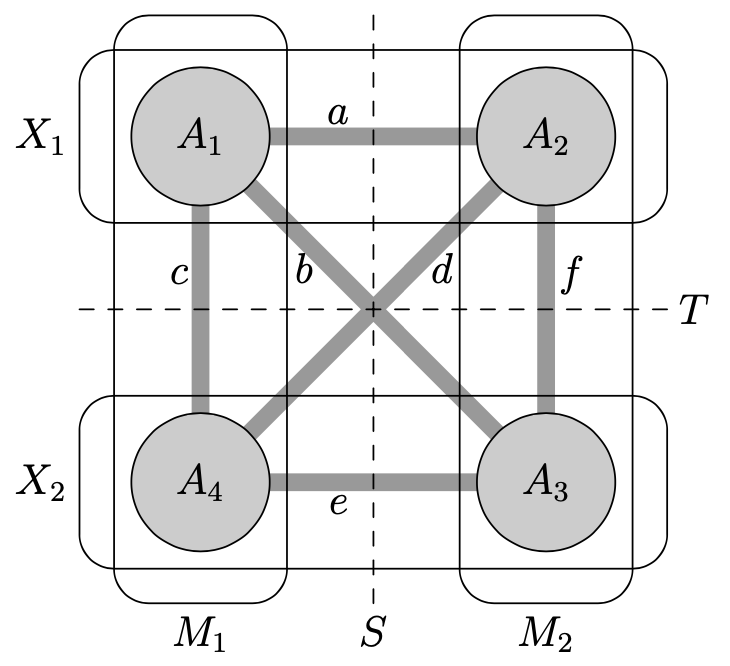
\includegraphics[width=0.5\linewidth]{graphs/rajnik-cyclic-part-junction-illustration}
		\caption{\cite{Rajnik_phd} Intersecting cuts S and T in the graph G}
		\label{fig:rajnik-cyclic-part-junction-illustration}
	\end{figure}
	
	Next let $r_i=|\delta(A_i)|$ for each $i\in\{1,2,3,4\}$. We can see that each of such $r_i$ is determined by the values of $a,b,c,d,e$ and $f$, for instance $r_1=a+b+c$. We prove by contradiction that each of $A_1, A_2,A_3$ and $A_4$ is non-empty. Suppose that some $A_i$ for $i\in\{1,2,3,4\}$ is empty. Then $M_1$ or $M_2$ would contain the whole cyclic $l$-pole $X_1$ or $X_2$, contradicting the assumption about $M_1$ and $M_2$.
	
	From the sizes of $S$ and $T$ we know that
	\begin{align}
		a+b+d+e &= k, \label{abde_eq_k}\\
		l=c+b+d+f &< k. \label{cbdf_smaller_k}
	\end{align}
	
	We now show that for each $i\in\{1,2,3,4\}$ at least one of the inequalities $r_i\geq k$ or $r_{i+1}\geq k$ is true, taking the indices modulo 4. Suppose to the contrary that there exists such $i\in\{1,2,3,4\}$ for which $r_j\leq k-1$ for both $j\in\{i, i+1\}$. Let us look at the properties of one of such $A_j$. We know that it contains less than $k$ semiedges, say $m$. We prove that is must be acyclic by contradiction. Let $A_j$ be in $M_1$, the proof for $M_2$ is analogous. Suppose that it would contain a cycle. Then $A_j$ would be a cyclic $m$-pole with $m<k$, contained in $M_1$, contradicting the assumption about $M_1$. Thus, we have that $|A_j|\leq r_j-2\leq k-3$ for both $j\in \{i, i+1\}$. By denoting $M$ as $G[A_i\cup A_{i+1}]$ we have $|M|\leq 2k-6$ ($A_i$ and $A_{i+1}$ are vertex disjoint). Note that $M$ is by its definition one of the multipoles $X_1, X_2, M_1,$ or $M_2$. This means that $M$ is cyclic and $|M|\geq k$ due to the girth of $G$ which must be at least $k$. From $k\leq |M|\leq 2k+6$ we have $k\geq 6$ so by the assumption of the theorem $M_1$ and $M_2$ are different from the $k$-cycle. Also both of $X_1$ and $X_2$ are different from $k$-cycles since they have less than $k$ semiedges. Therefore $M$ is not a $k$-cycle and it is a cyclic multipole with at most $k$ semiedges and girth at least $k$, so by \cref{lem:rajnik5.1}, $|M| \geq 2k - 4$, contradicting the fact that $|M|\leq 2k-6$.
	
	Thus for each $i\in\{1,2,3,4\}$ we have $r_i\geq k$ or $r_{i+1}\geq k$, from which it follows that
	\begin{align}
		r_1 =a+b+c\geq a+b+d+e=k \text{ and } r_3 =b+e+f \geq a+b+d+e=k\label{r1r3}
	\end{align}
	
	or
	\begin{align}
		r_2 =a+d+f \geq a+b+d+e=k \text{ and } r4 =c+d+e\geq a+b+d+e=k\label{r2r4}
	\end{align}
	
	is true. After summing, Inequalities \cref{r1r3} imply that $c+f\geq a+2d+e\geq a+e$ and Inequalities \cref{r2r4} imply that $c+f\geq a+2b+e\geq a+e$. In both cases we have obtained $c+f\geq a+e$. However by Inequality \cref{cbdf_smaller_k} we have 
	$$l=b+c+d+f<a+b+d+e=k$$
	
	so $c+f<a+e$, leading to a contradiction.
	
	We see that there is no cycle separating edge cut in $G$ with less than $k$ edges. Also there is the cycle-separating $k$-edge-cut $S$, thus it must be minimal and $\zeta(G)=k$.
	
	If the girth of $G$ would be less than $k$, then $\zeta(G)<k$ as well, because of \cref{prop:cyclic-con-less-than-girth}.
\end{proof}

A corollary of this theorem is that in this case the cyclic $k$-poles $M_1$ and $M_2$ are cyclic $k$-parts.

If we would be able to construct a cyclic $k$-pole for each $k$, such that it contains a cycle, has girth at least $k$ and does not create short cycles when connected to another cyclic $k$-pole, we could make it easier to decide if given cyclic $k$-pole is a cyclic $k$-part. If it does not contain a cyclic $l$-pole such that $l<k$, the \cref{th:junction-of-kpoles-cyclic-edge-connectivity} can be applied and thus it would be a cyclic $k$-part. However we first need to find such cyclic $k$-poles for each $k$. \todo{spomeň asi nejak adjuncts}

\begin{lemma}\label{lem:cyclic-k-pole-no-short-cycles-exists}
	For each $k\geq 1$, there exists a cyclic $k$-pole with the following properties:
	\begin{enumerate}
		\item The girth is at least $k$,
		\item It contains no cyclic $l$-pole for any $l<k$,
		\item The distance between any pair of semiedges is at least $k-2$.
	\end{enumerate}
\end{lemma}

\begin{proof}
	For $k$ equal to 1 and 2 we see that $C_k$ fulfills the requirements, we shall only explore $k\geq 3$. For given $k$ we construct a cubic Cayley graph with girth $2k$ according to \cref{th:cayley-girth-regular}. Let us denote this graph as $G$. Then $\zeta(G)=2k$ by utilizing \cref{th:cyclic-connectivity-of-transitive}. Next let $P$ be a path of length $k-3$ in $G$. Since $k\geq 3$ and $|V(G)|$ is evidently at least $2k$, there will always be such path. Remove all of the vertices on this path along with all isolated edges which were created and denote the result as $G'$. Since by removing some vertices and edges from a graph it is not possible to lower a girth, or introduce a new smaller cyclic $l$-pole, we must prove only the third condition about the distance between the semiedges. To be precise, we need to prove that
	\begin{enumerate}
		\item $G'$ is a cyclic $k$-pole,
		\item the distance between any pair of semiedges in $G'$ is at least $k-2$.
	\end{enumerate}
	The latter is easier to prove. Suppose that there are two semiedges $s_1$ and $s_2$, such that $d(s_1,s_2)=l<k-2$. Let us denote the shortest path between them as $Q$. Before removing the vertices in $G$, these edge ends were incident with vertices $v_1$ and $v_2$ respectively, not necessarily different. Since $v_1$ and $v_2$ lie on $P$, it holds that $d(v_1,v_2)\leq k-3$, let us denote the shortest path as $P'$. Now let $e_1$ and $e_2$ be the edges containing the edge ends which became semiedges $s_1$ and $s_2$ respectively. Then $e_1Qe_2P'$ is a closed path of length at most $2+(k-2)+(k-3)=2k-3$, contradicting the fact that $G$ has girth $2k$. \todo{ilustrovať} 
	
	Now we shall prove that $G'$ is a cyclic $k$-pole, meaning it contains a cycle and has $k$ semiedges. 
	
	We first prove that $\delta(G')=2$, proving it contains a cycle. Suppose that there is a vertex $v$ in $G'$ with degree less than two. We see that there is no pair of vertices in $G$ for which are connected by multiple edges, then the girth would be at most two, which would contradict the fact that $k\geq 3$ and the girth of $G$ is $2k$. Thus at least two distinct neighbors of $v$ were removed from $G$ during the creation of $G'$. Let these neighbors be $w_1$ and $w_2$. Since they lie on a path $P$ of length $k-3$, the distance between them is at most $k-3$. Let us denote the shortest path between them as $P'$. Let $e_1$ and $e_2$ be edges connecting $v$ to $w_1$ and $w_2$ in $G$ respectively. Then $e_1P'e_2$ is a cycle of length at most $k-1$ in $G$, contradicting the fact that $k\geq 3$ and the girth of $G$ is at least $2k$.
	
	Finally, we prove that the result has $k$ semiedges. Note that no two non-adjacent vertices on the path $P$ can be connected by an edge, as this would create a cycle of length at most $k-2$, contradicting our assumption.
	
	On path of length $k-3$ there are $k-2$ vertices. If $k=3$, we just remove one vertex and it is evident that the result will have three semiedges \todo{ilustrácia}. If $k > 3$, there are two end vertices of the path and $k-4$ internal. Each internal vertex results in one semiedge in $G'$ after its removal, since two of its neighbors are removed as well and the third neighbor must be some vertex outside $P$. The end vertices result in two semiedges in $G'$ after their removal, since only one of their neighbor is removed. Thus the number of semiedges in $G'$ will be $2\cdot 2 + (k-4)=k$, proving that $G'$ will have k semiedges.
\end{proof}

We will denote the cyclic $k$-poles constructed this way as $W_k$.

\begin{theorem}\label{th:alternative-definition-of-cyclic-part}
	Let $M$ be a cyclic potentially cyclically $k$-connected $k$-pole. Then $M$ is a cyclic $k$-part.
\end{theorem}

\begin{proof}
	Since each $k$-cycle $C_k$ is a cyclic part as proven in \cref{lem:each-cycle-cyclic-part} we can assume that $M$ is different from a cycle. Let $W_k$ be a cyclic $k$-pole satisfying \cref{lem:cyclic-k-pole-no-short-cycles-exists} and let $G$ be a junction $M*W_k$. We prove that $G$ has girth at least $k$. Suppose by contradiction that $g(G)<k$. Let us denote the shortest cycle in $G$ as $C$, $|C|=l\leq k-1$. There are multiple possibilities of where the cycle is located, we shall explore all of them.
	\begin{enumerate}
		\item $C$ is contained in $M$. Since $|C|=l$ and $M$ is cubic, $M$ contains the $l$-pole $C_l$ as well, contradicting the assumption.
		\item $C$ is contained in $W_k$. This leads to a contradiction, since we have constructed $W_k$ in a way that it has girth at least $k$.
		\item $C$ is not contained in neither, instead it was created after the junction $M*W_k$. Let the cycle be $ePfQ$, where $e$ and $f$ are edges resulting from the junction $M*W_k$, $P$ are edges inside $W_k$ and $Q$ is the rest of the edges of the cycle. However since the distance of any two semiedges in $W_k$ is at least $k-2$, it holds that $|P|\geq k-2$ and thus $|ePf|\geq k$, contradicting the fact that the cycle is shorter than $k$.
	\end{enumerate}

	Since all cases lead to a contradiction it holds that $g(G)\geq k$. Thus we see that $G$ is a cyclic cubic graph with girth at least $k$, resulting from the junction $M*W_k$. Since both $M$ and $W_k$ do not contain a cyclic $l$-pole for $l<k$, both are different from a cycle of length $k$ and their junction $G$ has girth at least $k$, we can apply \cref{th:junction-of-kpoles-cyclic-edge-connectivity} and conclude that $\zeta(G)=k$. Because of this fact we have proved that $M$ is in fact a cyclic $k$-part.
\end{proof}

\todo{Zamyslenie nad algoritmom na zisťovanie/generovanie cyklických častí}

\section{Junctions of multiple multipoles}

\begin{lemma}\label{le:junction-two-no-small-girth}
	Let $M_1$ and $M_2$ be cyclic, potentially cyclically $k$-connected and cyclically nontrivial $k$-poles. Let $m_i$ be the size of the smallest potentially cycle separating cut in $M_i$. Let $G$ be the junction of $M_1$ and $M_2$. If $m_1+m_2\geq k$ then $g(G)\geq k$. \todo{tie požiadavky znejú hrozne, nejak to modifikovať...}
\end{lemma}

\todo{túto lemu asi vieme generalizovať aj nie len že to sú k-póly, ale ľubovoľné potenciálne cyklicky súvislé a nemusí to byť junction ale aj partial junction}

\begin{proof}
	\todo{} suppose the girth is smaller than k. If $k=1$, then there is no new cycle after the junction and the girth is okay (contradiction). If $k\geq 2$, then the shortest cycle must go through two of the new edges. Since both multipoles are cyclic, we have to cut this new cycle out from both of them, and thus we need to cut at least $m_1+m_2$ edges leading to a contradiction. \todo{Pozor ale že nemusíme robiť cut, možno to vedia byť hocijaké k-póly, nie len cyklické. Princíp je ten, že ide cez aspoň 2 nové hrany (vie aj viac), ale ak musíme dačo orezať tak to bude aspoň $m_i$, pozor ešte na independent}
\end{proof}

\begin{lemma}\label{lem:cyclic-multipoles-with-girth-and-distance}
	Let $M_1$ and $M_2$ be multipoles with girth at least $k$. Let $d_i$ be the minimal distance between any pair of semiedges in $M_i$. Let $M$ be a partial junction $M_1*M_2$. If $d_1+d_2\geq k-2$ then $g(M)\geq k$.
\end{lemma}

\begin{proof}
	Suppose that the girth of $M$ is less than $k$. Since both $M_1$ and $M_2$ have girth at least $k$, any shortest cycle must use edges from both multipoles, necessarily crossing between them at least twice.
	
	Let $e_1,\dots,e_j$ denote the edges in $M$ that were created by the partial junction between $M_1$ and $M_2$. Consider a shortest cycle $C$ in $M$. This cycle must:
	
	\begin{enumerate}
		\item Enter $M_1$ through some edge $e_1$ and leave through another edge $e_2$, following a path $P$ in $M_1$,
		\item After entering $M_2$ through $e_2$, leave through an edge $e_3$ (which may or may not be $e_1$), following a path $Q$ in $M_2$.
	\end{enumerate}

	Thus, a part of cycle $C$ contains the path $e_1Pe_2Q$. Observe that the path $P$ represents a path between a pair of semiedges in former $M_1$, similarly $Q$ in $M_2$. Thus by definition of $d_1$ and $d_2$:
	
	\begin{enumerate}
		\item Path $P$ has length at least $d_1$,
		\item Path $Q$ has length at least $d_2$,
		\item The edges $e_1$ and $e_2$ contribute length 2.
	\end{enumerate}

	Therefore, the total length of this path is at least $2+d_1+d_2 \geq 2+(k-2) = k$, contradicting our assumption that $M$ contains a cycle shorter than $k$.
\end{proof}

\begin{lemma}\label{lem:size-of-minimal-potentially-cycle-separating-after-junction}
	Let $M_1$ and $M_2$ be cyclically nontrivial multipoles, such that $m_1$ and $m_2$ are the sizes of minimal potentially cycle separating cuts in $M_1$ and $M_2$ respectively. Let $M$ be the result of a partial junction $M_1*M_2$ of size $j$. Then the size of the minimal potentially cycle separating cut in $M$ is at least $\min\{m_1,m_2,j\}$.
\end{lemma}

\begin{proof}
	Suppose that the minimal potentially cycle separating cut in $M$ has size $m_X$ and it holds that $m_X<\min\{m_1,m_2,j\}$. Let us denote this cut as $X$. First suppose that $j=1$. This means that $m_X$ must be 0, however since the resulting graph is connected \todo{treba dokázať?} this leads to a contradiction.
	
	Now suppose that $j=2$. Since we have shown that the case $m_X=0$ leads to a contradiction, we shall look at $m_X=1$. By cutting one of the two new edges which were created by the partial junction we will not disconnect the graph, the cut must be an edge from $M_1$ or $M_2$. Suppose it is in $M_1$. We can see that this edge must be a bridge, since by cutting it we disconnect the graph. If $M_1$ has at least three semiedges, it is evident that this cut is potentially cycle separating, which leads to a contradiction with the fact that $m_X<m_1$. For this to not be a potentially cycle separating cut it must hold that $M_1$ has two semiedges and the shortest path between them goes though this bridge \todo{ilustrácia -O-O-}. However this is not an edge cut in $M$. If we select one vertex from each component of $M_1$ after cutting this edge, we can still find a path between them \todo{lepšie dokázať, formálne cez tie paths}. This means that $X$ is not a cut in $M$, leading to a contradiction.
	
	At last we shall explore the case where $j\geq 3$. This means, that both $M_1$ and $M_2$ have at least three semiedges. As in the case above, we see that since $m_X<j$ we do not disconnect the graph just by cutting the edges created by the partial junction, thus the cut needs to contain some edges originally from $M_1$ or $M_2$. Suppose that it contains edges from $M_1$. This means that the edges in the cut from $M_1$ are an independent edge cut in $M_1$ \todo{znova, treba asi dokázať.} However since $M$ has at least three semiedges, it must hold that in at least one of the components there will be at least two semiedges, meaning that this cut would be potentially cycle separating in $M_1$ and smaller than $m_1$, leading to a contradiction.
	
	\todo{Treba asi ukázať nie len že to sú rezy v $M_i$, ale aj že sú independent, teda potentially cycle separating.}
\end{proof}

\begin{theorem}\label{th:connecting-potencially-k-connected}
	Let $M_1$ and $M_2$ be connected and potencially cyclically $k$-connected multipoles with the same number of semiedges, which do not contain an independent edge cut of size $a$, such that after the cut there is an acyclic component with $b$ former semiedges (not resulting from the cut) and $b>a$. Let $m_1$ and $m_2$ be the sizes of minimal potentially cycle separating cuts in $M_1$ and $M_2$ respectively. If $m_1+m_2\geq k$ then the partial junction $M=M_1*M_2$ is potencially cyclically $k$-connected unless $M$ has less than $k$ semiedges. (Nie je to úplne formálne, to potom prepíšem)
\end{theorem}

\begin{proof}
	Notes:
	\begin{itemize}
		\item Contradiction - there is an $l$-pole $X$ with $l<k$. Let this $l$-pole have the smallest $l$ and is the largest possible (number of edges, or some inclusion, does not really matter imo.)
		\item $A_1,\cdots$ the illustration same as before, however $x_i$ equals semiedges from $A_i$.
		\item We prove that $M-X$ contains a cycle. We can easily prove that it is non-empty, if it was empty then $M=X$ and $M$ would have less than $k$ semiedges ($l$ to be precise) leading to a contradiction.
		
		Now, suppose that $M-X$ does not contain a cycle, thus is a forest. Let's look at any tree in this forest, $T$. The tree contains $a$ semiedges resulting from the cut and $b$ former semiedges. If $b\leq a$ it would lead to a contradiction that $X$ has the least semiedges and is the largest possible, by not cutting out this tree we would obtain $X'$ with at most semiedges as $X$ and larger. Thus $b>a$. 
		
		If the whole tree was part of $M_1$ or $M_2$ this directly leads to a contradiction. Thus suppose that this tree contains parts from $M_1$ and $M_2$. Let $b_1$ be semiedges incident to vertices from $M_1$ in $b$ and $a_1$ similarly from $a$. For $M_2$ we have $a_2$ and $b_2$. Since $b=b_1+b_2, a=a_1+a_2$ and $b>a$, it must hold that $b_1>a_1$ or $b_2>a_2$. Suppose $b_1>a_1$. Then (and this will be hard to formulate :D) if we cut out only the vertices from $M_1$ from $T$, we would obtain an acyclic component formerly part of $M_1$. The new semiedges resulting from the cut are former semiedges from $M_1$, since they became edges after the junction with $M_2$, thus they are type ''b'' vertices. Let the number of these semiedges be $b'_1$. Now we have an acyclic component from $M_1$ with $b'_1+b_1$ former semiedges, and cut out by $a_1$ edges, such that $b'_1+b_1>a_1$ (since $b_1>a_1$) contradicting the assumption by $M_1$. (This is needed to be formulated better, however the main idea should be captured there).
		
		\item We shall prove that all $A_i$ are non-empty. $A_1$ and $A_2$ are easy, otherwise the whole $l$-pole is in $M_1$ or $M_2$.
		\item $A_3$ and $A_4$ can't be empty in the same time because $M$ has $k$ or more semiedges (we have proved it before).
		\item Suppose $A_3$ is empty, then the whole $M_2$ is contained in $X$. We then prove that $M-X$ is a cyclic $j$-pole with $j\leq l < k$, and contained in $M_1$ leading to a contradiction. We know that $M-X$ has a cycle, and number of its semiedges is in this case $c+d+x_4$, since $A_3$ is empty. Also we know that $x_1+x_4=x_2$ since $M_1$ and $M_2$ have the same number of semiedges. We then know that $c+d+x_1+x_2<k$, and $x_4\leq x_2$ since $x_1+x_4=x_2$. From this we get $c+d+x_1+x_4<k$, and thus $c+d+x_4<k$, contradicting the fact that $M_1$ is potencially cyclically $k$-connected. Same goes for empty $A_4$.
		\item Then we must prove that $a$ is at least 2. If it was 0, then there would be a cyclic pole with less than $l$ semiedges in $M_1$ or $M_2$. If it was 1, then there would be a cycle in $A_1$ or $A_2$. Suppose it is in $A_1$. We know that $c+b+d+f+x_1+x_2<k$. Then $f\geq 1$ since $M_2$ is connected and $a=1$ thus $a\leq f$ and thus $c+b+d+a+x_1+x_2<k$. From this we see that $a+b+c+x_1<k$, meaning $A_1$ would be a cyclic $j$-pole with $j<k$ in $M_1$, leading to a contradiction. \todo{maybe separate this in some separate lemma, so we will not repeat the proof in multiple theorems}
		\item The cut separating $X$ from $M-X$ is independent. This can be easily proven, if it was not independent we could obtain $X'$ with less semiedges, however we should put it in the proof.
		\item Because of this for $c$ and $f$ it must hold that $c+f\geq k$. They are cuts in $M_1, M_2$ because all $A_i$ are non-empty and they are connected components. This leads to a contradiction with the fact that $c+b+d+f+x_1+x_2=l<k$.
	\end{itemize}
\end{proof}

PROBLEMS:

\begin{itemize}
	\item Veľa obmedzení, asi sa dá ešte zľahčiť požiadavka na $m_1,m_2$, aby ten druhý komponent bol ''problémový'', napr. nech obsahuje cyklus alebo aspoň 2 polhrany.
	\item Rovnako obmedzenie na rovnaký počet polhrán $M_1,M_2$.
	\item Obmedzenie na absenciu toho rezu ktorý nechá acyklický komponent.
	\item $S(M)$ môže byť aj 0, vtedy to je graf a platí to, len to asi treba niekde uviesť.
\end{itemize}

\todo{}We can also prove that there will be no problematic cut leaving the acyclic graph with more dangling edges than the cut size. Suppose that after the junction from the theorem above there will be a cut of size $a$, such that one of the components have $b$ former semiedges and $b>a$. The proof is basically in the theorem above, but we can formulate it in a separate lemma, and use it later during specific constructions. Also, we can use it then in the theorem proof, making the proof that $M-X$ contains a cycle easier (and the whole proof shorter ofc.)

\todo{PREDOBHAJOBY:}
\begin{itemize}
	\item Nájsť najmenší graf s cyklickou súvislosťou 7 (Mazák) - RIEŠENIE nie je to náhodou mcgee graph? Pre ten mi vyšla cykl. súvislosť 7 a je to najmenší graf kubický s obvodom 7 ((3,7)-cage). Každopádne viem vytvoriť nejaké stavebné bloky na stavanie cykl. 7-súvislých.
	\item Prípadne aj nájsť spôsob konštruovanie najmenších takých grafov, prípadne stavebných blokov na najmenšie.
\end{itemize}

\begin{theorem}\label{th:connecting-potencially-cyclically-connected-with-number-of-resulting-semiedges}
	Let $M_1$ and $M_2$ be connected, cyclically nontrivial and potencially cyclically $k$-connected multipoles. Let $m_i$ be the size of the smallest potentially cycle separating cut in $M_i$. Let $M$ be a result of a partial junction $M_1*M_2$ of size $j$. Let us denote by $s_i$ the number of remaning semiedges after the partial junction in $M_i$, meaning $|S(M_i)|-j$. If $m_1+m_2\geq k$ and one of the following holds:
	
	\begin{enumerate}
		\item $s_1+s_2\geq k, m_1+s_2\geq k$ and $s_1+m_2\geq k$,
		\item $s_1+s_2=0$ thus $M$ is a graph,
	\end{enumerate}

	then $M$ is potentially cyclically $k$-connected.
\end{theorem}

\begin{proof}
	Suppose by contradiction that there is an $l$-pole $X$ in $M$, which has the smallest $l$ and from such is the largest. Let us denote the other component as $M-X$. Let $A_1,A_2,A_3,A_4$ denote the subgraphs of $G$ induced by $V(X_1)\cap V(M_1), V(X_1)\cap V(M_2), V(X_2)\cap V(M_2), V(X_2)\cap V(M_1)$ respectively. Let $a,b,c,d,e$ and $f$ denote the number of edges connecting $A_1$ and $A_2$, $A_1$ and $A_3$, $A_1$ and $A_4$, $A_2$ and $A_4$, $A_3$ and $A_4$, $A_2$ and $A_3$ respectively. Let $x_i$ be the number of dangling edges from $A_i$ as seen in \todo{ilustrácia}. By looking at the illustration we see that $b+c+d+f+x_1+x_2=l<k$
	
	We first prove that $A_1$ and $A_2$ are non-empty. Suppose that some $A_1$ is empty. Then $M_2$ would contain the whole cyclic $l$-pole $X$, contradicting the assumption about $M_2$.
	
	Next we prove that $A_3$ and $A_4$ cannot be empty at the same time. Suppose that both were empty, meaning $X=M$.
	\begin{enumerate}
		\item If it holds that $|S(M)|=0$, it would mean that $X$ is a 0-pole, however we need for $X$ to be a result from a cut, and we can not get a 0-pole this way.
		\item Otherwise this would mean that $|S(M)|=l<k$, contradicting the fact that $s_1+s_2\geq k$.
	\end{enumerate}

	Now let us look at the number of edges marked as $a$. If $a$ was 0, then there would be a cyclic pole with at most $l$ semiedges in $M_1$ or $M_2$, leading to a contradiction. If $a=1$, then there must be a cycle in $A_1$ or $A_2$. Suppose it is in $A_1$.
	\begin{enumerate}
		\item If $f=0$, then $A_3$ is empty (since $M_1$ and $M_2$ are connected) and $A_2=M_2$. Since $M_2$ is cyclically nontrivial, it has more than one semiedge meaning $x_2+d\geq 1$. This means, that $a\leq x_2+d$. Note that $e$ and $b$ must be 0 as well, since $A_3$ is empty. We know that $b+c+d+f+x_1+x_2<k$ and $a\leq x_2+d$, thus $a+b+c+f+x_1<k$. From this we see that $a+b+c+x_1<k$, meaning $A_1$ is a cyclic multipole with less than $k$ semiedges in $M_1$, leading to a contradiction.
		\item If $f\geq 1$, it holds that $a\leq f$ since we suppose that $a=1$. From $b+c+d+f+x_1+x_2<k$ we thus get $a+b+c+d+x_1+x_2<k$, from which it holds that $a+b+c+x_1<k$, again leading to a contradiction.
	\end{enumerate}
	We thus get that $a$ is at least two. The cut separating $X$ from $M-X$ is independent, since it is the minimal possible \todo{toto asi treba niekde dokázať, alebo spomenúť}. Now we shall explore $A_3$ and $A_4$. If both are non-empty, $c$ and $f$ are at least 1, and since $a\geq 2$, they must be potentially cycle separating cuts, meaning $c\geq m_1$ and $f\geq m_2$. However $m_1+m_2\geq k$, thus $c+f\geq k$, contradicting the assumption that $b+c+d+f+x_1+x_2<k$.
	
	Now suppose one of $A_3$ and $A_4$ is empty, say $A_3$.
	
	\begin{enumerate}
		\item If $|S(M)|=0$, then this would mean that $A_4$ is a cyclic $l$-pole in $M_1$, leading to a contradiction \todo{treba dokázať že je cyklický?}.
		\item Otherwise $c$ represents a potentially cycle separating cut since $a\geq 2$, thus $c\geq m_1$. Also we see that $x_3=0$ and thus $x_2=s_2$. Since $m_1+s_2\geq k$, it holds that $c+x_2\geq k$, contradicting the assumption that $b+c+d+f+x_1+x_2<k$.
	\end{enumerate}
\end{proof}

\subsection{Examples}

First construction is the junction of 3 potencially 5-connected cyclic 5-poles along with one point in the middle.

\begin{example}
	Suppose we want to connect three 5-poles, along with one point in the middle, and we want to decide whether the result is cyclically 5-connected. The illustration can be seen in \cref{fig:3-5-poles-connected}. We can put some requirements on the connected 5-poles, and by utilizing proved theorems we can prove that in these cases, the result will in fact be potentially cyclically 5-connected.
	
	\begin{figure}
		\centering
		\begin{tikzpicture}
			% Big nodes (triangle vertices)
			\node[circle, draw, fill=white, minimum size=15pt] (A) at (0,2) {};
			\node[circle, draw, fill=white, minimum size=15pt] (B) at (-1.5,0) {};
			\node[circle, draw, fill=white, minimum size=15pt] (C) at (1.5,0) {};
			
			% Center node
			\node[circle, draw, fill=black, minimum size=5pt, inner sep=0pt] (D) at (0,0.7) {};
			
			% Parallel edges between triangle vertices
			\draw (A.-120) -- (B.50)  (A.-140) --(B.70);
			\draw (A.-40) -- (C.120)  (A.-60) --(C.140);
			\draw (B.-10) -- (C.190)  (B.10) --(C.170);
			
			% Edges from center to triangle vertices
			\draw (D) -- (A);
			\draw (D) -- (B);
			\draw (D) -- (C);
		\end{tikzpicture}
		\caption{TODO}
		\label{fig:3-5-poles-connected}
	\end{figure}
	
	Let $M_1,M_2,M_3$ be potentially cyclically 5-connected 5-poles, with sizes of their minimal potentially cycle separating cuts $m_1,m_2,m_3$ respectively, such that $m_1\geq 2,m_2\geq 3$ and $m_3\geq 3$ as illustrated in \todo{figure}.
	
	In the first step, we perform a partial junction of size two on $M_1$ and $M_2$ as illustrated in \todo{figure}. By \cref{th:connecting-potencially-cyclically-connected-with-number-of-resulting-semiedges} the result is potentially cyclically 5-connected, let us denote it as $M_{12}$. About its minimal potentially cycle separating cut we know that $m_{12}\geq 2$ by utilizing \cref{lem:size-of-minimal-potentially-cycle-separating-after-junction}. It can be observed that the size of the cut is exactly two.
	
	Now we perform a partial junction with the singular point and $M_{12}$ resulting in $M'$ as shown on \todo{ilustrácia}. Since it is cyclically trivial, we can not utilize any of the theorems proved so far. Because of this, we have to prove that the result will be potentially cyclically 5-connected.
	
	Suppose it is not, let $X$ be a cyclic $l$-pole in $M'$ for $l<5$, with the least semiedges and the largest from those. We know that $X$ must contain the added point, otherwise it would be present in $M'$ and would contradict the fact that it is potentially cyclically 5-connected. Also it must contain both neighbors of the newly added point, otherwise we could obtain a cyclic multipole with less than $l$ semiedges, as it is visible in \todo{figure}. Let $e_1,e_2$ be the two edges which were created by the partial junction of $M_1$ and $M_2$, as visible in \todo{figure}.  It must hold that $M-X$ is non-empty, otherwise $X=M$ and it would contradict the fact that $X$ has less than 5 semiedges.
	\begin{enumerate}
		\item First suppose that at least one edge from $e_1,e_2$ is in $X$. If $X$ contains the whole $M_2$, then $X$ has at least $2+1+m_1$ semiedges, that is because $M_2$ has two semiedges, the added point has one, and since we need to perform a cut in $M_1$ which leaves two former semiedges, the size must be at least $m_1$. Since $m_1\geq 2$, it holds that $X$ has at least 5 semiedges, leading to a contradiction. Thus it means that $X$ does not contain whole $M_2$. Similarly if $X$ would contain the whole $M_1$, we would get that $X$ has at least $2+1+m_2$ semiedges, that is at least 6, leading to a contradiction. Thus it does not contain whole $M_1$ and neither $M_2$, meaning it cuts out two former semiedges from both, thus $X$ has at least $m_1+m_2+1$ semiedges, which is at least 6, leading to a contradiction.
		\item Now suppose that $X$ does not contain $e_1$ and neither $e_2$. This means that the cycle in $X$ must be whole in $M_1$ or $M_2$, suppose it is in $M_1$. Now, modify $X$ in a way, that we will keep only the vertices originally from $M_1$ as showcased in \todo{figure}, resulting in $X'$. There will be a new semiedge, resulting from cutting the edge connecting $M_1$ to the new vertex, however we will remove the semiedge from the added point, as well as all semiedges from the vertices in $M_2$, which means that $X'$ has at most semiedges as $X$. This leads to a contradiction, since $X'$ would be a cyclic multipole with less than $k$ semiedges in $M_1$.
	\end{enumerate}

	We have proved that after adding the point the resulting multipole $M'$ is potentially cyclically 5-connected. The size of the minimal potentially cycle separating cut in $M'$ will still be at least two, since we have not created a bridge.
	
	At last, we perform a junction of $M'$ and $M_3$ forming $G$. By \cref{th:connecting-potencially-cyclically-connected-with-number-of-resulting-semiedges} and the case where $|S(G)|=0$ it holds that $G$ is potentially cyclically 5-connected, meaning it is cyclically 5-connected by \cref{lem:graphs-potential-and-normal-cyclic-connected-eq}.
\end{example}

\textbf{Second thing is the connection of 4 6-poles.}

\begin{enumerate}
	\item We first say that all 4 6-poles must have the smallest $m_i$ cut at least 3 and be potencially cyclically $6$-connected.
	\item We connect two of them creating 2 new edges. By \cref{th:connecting-potencially-cyclically-connected-with-number-of-resulting-semiedges} the result is potencially cyclically $6$-connected.
	\item We do the same thing with remaining two.
	\item We prove that the distance between any pair of semiedges in both components is at least $m_i-1$, thus 2.
	\begin{enumerate}
		\item Let $r,s$ be two semiedges and let $P$ be the shortest path between them.
		\item First suppose that they are in the same former multipole.
		\item The former component can not be acyclic, since then $m_i$ would be $\leq 1$ contradicting assumption that it is at least 3.
		\item If it was cyclic, it cannot be a cycle $C_l$ with $l\geq 6$ (because of the girth), because then the minimal cut would be $2$. Thus we can cut out the path from the rest of the multipole. However we then would need to cut at least $3$ edges because of $m_i$, thus the distance would be at least 2.
		\item If each semiedge is in different former multipole, the shortest path must go through some created edge $e$, Let $P'$ be the part in one of the multipoles. Then we can repeat the proof, since we would need to cut out a former semiedge $t$ which was junctioned to form an edge, and this would mean that $P'$ is at least 2, so $P$ must be at least 2.
	\end{enumerate}
	\item We connect these two multipoles to form the result and by utilizing \cref{lem:cyclic-multipoles-with-girth-and-distance} we see that the girth is at least $6$.
	\item Now by \cref{th:junction-of-kpoles-cyclic-edge-connectivity} the result is cyclically 6-connected.
\end{enumerate}


Next things are the \textit{superpositions} (or smth like that) which we were discussing on the meeting about the thesis. We have multiple 7-poles which are potentially cyclically 7-connected and we are connecting them in a circle, such that we connect each two by partial junction of size 3. In the end, the result will be potentially cyclically 7-connected if we connect at least 7 of them.

We say that we need at least one with minimal potentially cycle separating cut 3 and others with 4.

\begin{enumerate}
	\item We first connect the one with three to the one with 4. By using \cref{th:connecting-potencially-cyclically-connected-with-number-of-resulting-semiedges} we obtain a potentially cyclically 7-connected multipole with the minimal potentially cycle separating cut of size 3 by \cref{lem:size-of-minimal-potentially-cycle-separating-after-junction}.
	\item We connect more and more, using the mentioned theorem and lemma.
	\item In the end we finish the circle. \todo{problem - the size $s_2$ of the connected multipole will be just 1 in this case. Thus we can't really use this theorem... We shall look into how to fix it.}
\end{enumerate}

\section{Creating potentially cyclically $k$-connected multipoles}

\todo{}

\chapter{Cyclic part Inflations}

We can extend the definition of inflations, by allowing expanding each vertex of the original graph into a cyclic $k$-part, where $k$ is the degree of the respective vertex.

\todo{Definovať kedy vrcholy korešpondujú cyklickej časti v grafe, teda keď pospájam cyklické časti $P_1,\cdots, P_n$ do výsledku $G$, tak kedy nejaká množina vrcholov $V$ korešponduje v $G$ s $P_i$. Resp. treba to definovať?}

\begin{definition}
	\label{def:cyclic-part-inflation}
	Let $G$ be a graph and let $H$ be a cubic graph resulting from performing partial junctions on cyclic parts $P=\{P_1,\cdots,P_n\}$. Let $V=\{V_1,\cdots, V_n\}$ be a partition of $V(H)$ such that for each $i$ from 1 to $n$ the set $V_i$ corresponds to the cyclic part $P_i$. Then $H$ is called a \textit{cyclic part inflation} of $G$ if the graph obtained from $H$ by contracting each set $V_i\in V$ into a single vertex is isomorphic to $G$. The set of all cyclic part inflations of $G$ is denoted by $I_P(G)$.
\end{definition}

For inflations it has been proved, that in specific cases if the original graph is $k$-connected, then each of its inflations is cyclically $k$-connected. First observation about these cyclic part inflations is in the form of a lemma, and is basically saying, that cyclic edge-connectivity of the inflation is bounded from above by the edge-connectivity of the former graph.

\begin{lemma}
	Let $G$ be a nontrivial graph with $\lambda(G)=k$. Then for each $H\in I_P(G)$ it holds that $\zeta(H)\leq k$.
\end{lemma}

\begin{proof}
	Let $S$ be the smallest edge-cut in $G$ separating it into components $M_1$ and $M_2$, and $G'$ be a cyclic part inflation from $I_P(G)$. In $G'$ this edge cut is cycle separating, since there is at least one cycle in each component which arose after the cyclic part inflation, and is of size $k$, thus the smallest cycle separating cut in $G'$ must be of size at most $k$.
\end{proof}

Similar to \cref{th:inflations-cyclic-connectivity}.

\begin{theorem}
	Let $k\geq 3$ and let $G$ be a $k$-connected graph with girth at least $k$. Then every  $H\in I_P(G)$ is cyclically $k$-edge-connected.
\end{theorem}

\begin{proof}
	Let $H\in I_P(G)$. For each vertex $v\in V(G)$, denote the unique cyclic part in $H$ corresponding to it (as in \cref{def:cyclic-part-inflation}) by $P_v$. We say that a cycle $C$ in $H$ is \textit{traversal} if there are two distinct vertices $v_1,v_2$ in $G$ with $V(P_v)\cap V(C)\neq \emptyset$ for both $v\in\{v_1,v_2\}$, so it goes through two unique cyclic parts in $H$. Otherwise we say that $C$ is \textit{non-traversal}, meaning $C\subseteq P_v$ for some $v\in V(G)$. \todo{túto definíciu dať do kapitoly o inflations}
	
	Suppose by contradiction, that $H$ is not cyclically $k$-edge-connected. Then $H$ has an edge cut $S$ with $|S|\leq k-1$ such that $H-S$ has precisely two components $D_1$ and $D_2$ and both contain a cycle.
	
	Let $D_i^G$ be the subgraph of $G$ induced by the vertex set $$\{x\in V(G)~|~ V(P_x)\cap V(D_i)\neq \emptyset\}$$
	so vertices from $G$, whose corresponding cyclic parts in $H$ have at least one vertex overlapping with the component $D_i$. Let us define sets $S_V^G$ and $S_E^G$ as
	\begin{align*}
		S_V^G &= \{x\in V(G) ~|~ E(P_x)\cap S\neq \emptyset\} \\
		S_E^G &= \{e\in S ~|~ \forall x\in V(G): e\notin E(P_x) \}.
	\end{align*}
	
	This means, that $S_V^G$ are vertices from $G$ whose corresponding cyclic parts contain at least one edge from $S$ and $S_E^G$ are edges from $S$ which are not a part of any cyclic part, or in other words connect two vertices in $G$ and connect two cyclic parts in $H$. It can be seen that ${V(D_1^G)\cap V(D_2^G)=S_V^G}$, since the set contains vertices, whose corresponding cyclic parts contain edge from $S$, thus are split into the two components.
	
	It is evident that $S_V^G\cap S_E^G=\emptyset$, since one set contains vertices and the other one edges, meaning $|S_V^G\cup S_E^G|=|S_V^G|+|S_E^G|$. We prove that $|S_V^G\cup S_E^G|\leq |S|$. For each element $x\in S_V^G\cup S_E^G$ there is at least one representant in $S$, not overlapping with the representants of other elements. There are two possibilities for $x$:
	\begin{enumerate}
		\item The element $x$ is a vertex, thus $x\in S_V^G$. The representants in $S$ are in this case the links in $P_x$ which are in the edge-cut $S$. No other element from $S_V^G\cap S_E^G$ has overlapping representants, if it is some $y\in S_V^G$ different from $x$ it is evident that the links from $P_y$ will be different. On the other hand, if it is some $e\in S_E^G$, these elements have different representants, as it is explained next.
		\item The element $x$ is an edge, thus $x\in S_E^G$. Note that these are the edges from $S$, which are not a part of any cyclic part. For the sake of readability, len us denote it as $e$. The representant of $e$ in $S$ will be that edge itself. Same as before, no other element $y\neq e$ from $S_V^G\cap S_E^G$ has overlapping elements. If $y$ is from $S_V^G$, its representants are inner links from $P_y$, thus not containing $e$. If $y$ is from $S_E^G$, its representant is an edge different from $e$.
	\end{enumerate} 
	
	This means, that $|S_V^G\cup S_E^G|\leq |S|$, which means after putting everything together that $$|S_V^G|+|S_E^G|=|S_V^G\cup S_E^G|\leq |S|\leq k-1.$$
	
	Suppose that $V(D_i^G)-S_V^G\neq\emptyset$ for each $i\in \{1,2\}$, meaning there is a whole cyclic part in both $D_1$ and $D_2$. Then $G-S_v^G-S_E^G$ has two components $F_1^G$ and $F_2^G$. The number of vertex disjoint paths from a vertex of $F_1^G$ to a vertex of $F_2^G$ in $G$ is at most $|S_V^G|+|S_E^G|\leq k-1$, which contradicts by Menger's Theorem that $G$ is $k$-connected.
	
	Therefore we may assume without loss of generality that $V(D_1^G)-S_V^G=\emptyset$, meaning there is no whole cyclic part in $D_1$.
	
	Another thing to note is that in this case the component $D_2$ must contain at least one unsplit cyclic part, or in other words $V(D_2^G)-S_V^G\neq\emptyset$. Suppose that $V(D_2^G)-S_V^G=\emptyset$, which would mean that each cyclic part has been split by $S$. However $G$ is $k$-connected, thus $|V(G)|>k$ and since $S$ contains an edge from each of the cyclic parts it must hold that $|S|\geq |V(G)|>k$ which contradicts that $|S|\leq k-1$.
	
	By assumption $D_1$ contains a cycle, say $C_1$. Suppose that this cycle is non-traversal, thus $C_1\subseteq P_v$ for some $v\in V(G)$. It must hold that $v\in S_V^G$, since there is no unsplit cyclic part in $D_1$, meaning $P_v$ has been split by $S$. Let $V_1,$ and $V_2$ be the vertices from $P_v$ incident with a dangling edge in $D_1$ and $D_2$ respectively. Let $E_1$ and $E_2$ be the respective dangling edges. Let us denote the set $E_L(P_v)\cup S$ as $S_P$. This set contains the links from $P_v$ which were split by the cut $S$. By \cref{lem:cyclic-part-no-short-cut} it holds that $|S_P|\geq|E_2|$. Let us denote the set of links in $H$ from which result dangling edges in $E_2$ after severing edges from $S$ as $L_2$. We can now create an edge cut $S'=(S-S_P)\cup L_2$, which is cycle separating in $H$ and it holds that $|S'|\leq |S|\leq k-1$. Since both components now contain a whole cyclic part, this contradicts the assumption that $G$ is $k$-connected, as it was proved before.
	
	This means, that the cycle in $D_1$, say $C_1$ must be traversal. Thus $C_1$ corresponds to a closed trail in $D_1^G$, say $C_1^G$. Since the girth of $G$ is at least $k$ and every closed trail contains a cycle, we have $|V(C_1^G)|\geq k$, which contradicts that $V(C_1^G)\subseteq V(D_1^G)\subseteq S_V^G$ and $|S_V^G|\leq k-1$.
	
\end{proof}

\chapter{Problems for further research}

\todo{}

\chapter*{Conclusion}
\addcontentsline{toc}{chapter}{Conclusion}
\markboth{Conclusion}{Conclusion}

% BIBLIOGRAPHY
\newpage
\thispagestyle{empty}

\bibliographystyle{unsrt}
\bibliography{references}

% APPENDICES
%\appendix
%\thesisappendices{}

\end{document}
